\documentclass{article}
\usepackage[a4paper, portrait, margin=1.1811in]{geometry}
\usepackage[dvipsnames]{xcolor}
\usepackage[english]{babel}
\usepackage[utf8]{inputenc}
\usepackage[T1]{fontenc}
\usepackage{helvet}
\usepackage{pgf-umlsd}
\usepackage{etoolbox}
\usepackage{amsfonts}
\usepackage{enumitem}
\usepackage{graphicx}
\usepackage{titlesec}
\usepackage{caption}
\usepackage{booktabs}
\usepackage{adjustbox}
\usepackage{subcaption}
\usepackage{multicol}
\usepackage{float}
\usepackage{amsmath}
\usepackage{listings}
\usepackage{tikz}
\usepackage[colorlinks, citecolor=cyan]{hyperref}

\usetikzlibrary{matrix,shapes,arrows,positioning,chains, calc}
\definecolor{dkgreen}{rgb}{0,0.6,0}
\definecolor{gray}{rgb}{0.5,0.5,0.5}
\definecolor{mauve}{rgb}{0.58,0,0.82}

\usepackage{caption}
\captionsetup[figure]{labelfont={bf},labelformat={default},labelsep=period,name={Figure }}	
% \captionsetup[table]{labelfont={bf},labelformat={default},labelsep=period,name={Table }}
\graphicspath{ {./images/} }
\usepackage{scrextend}
\usepackage{fancyhdr}
\usepackage{graphicx}
\newcounter{lemma}
\newtheorem{lemma}{Lemma}
\newcounter{theorem}
\newtheorem{theorem}{Theorem}

\fancypagestyle{plain}{
	\fancyhf{}
	\renewcommand{\headrulewidth}{0pt}
	\renewcommand{\familydefault}{\sfdefault}
	
}

%\pagestyle{plain}
\makeatletter
\setlength{\@fptop}{0pt}
\patchcmd{\@maketitle}{\LARGE \@title}{\fontsize{16}{19.2}\selectfont\@title}{}{}
\makeatother

\usepackage{authblk}
\def\code#1{\texttt{#1}}
\renewcommand\Authfont{\fontsize{10}{10.8}\selectfont}
\renewcommand\Affilfont{\fontsize{10}{10.8}\selectfont}
\renewcommand*{\Authsep}{, }
\renewcommand*{\Authand}{, }
\renewcommand*{\Authands}{, }
\setlength{\affilsep}{2em}  
\newsavebox\affbox
\author[1]{\textbf{Aarav Varshney}}
% \author[2]{\textbf{Mahabir Prasad Jhanwar}}
\affil[1]{\textbf{Ashoka University}, \texttt{aarav.varshney@alumni.ashoka.edu.in}}
% \affil[2]{\textbf{Ashoka University}, \texttt{mahavir.jhawar@ashoka.edu.in}
% }

\titlespacing\section{0pt}{12pt plus 4pt minus 2pt}{0pt plus 2pt minus 2pt}
\titlespacing\subsection{12pt}{12pt plus 4pt minus 2pt}{0pt plus 2pt minus 2pt}
\titlespacing\subsubsection{12pt}{12pt plus 4pt minus 2pt}{0pt plus 2pt minus 2pt}


\titleformat{\section}{\normalfont\fontsize{10}{15}\bfseries}{\thesection.}{1em}{}
\titleformat{\subsection}{\normalfont\fontsize{10}{15}\bfseries}{\thesubsection.}{1em}{}
\titleformat{\subsubsection}{\normalfont\fontsize{10}{15}\bfseries}{\thesubsubsection.}{1em}{}

\titleformat{\author}{\normalfont\fontsize{10}{15}\bfseries}{\thesection}{1em}{}

\title{\textbf{\huge Report on TLS 1.3}\\}
\date{}    

\begin{document}

\pagestyle{headings}	
\newpage
\setcounter{page}{1}
\renewcommand{\thepage}{\arabic{page}}

\setlength{\parskip}{0.5em}
	
\maketitle
	
\noindent\rule{15cm}{0.5pt}
	\begin{abstract}
        The Internet Engineering Task Force (IETF) formed the Transport Layer Security (TLS) working group to develop a standardized SSL-like protocol. In 1999, the group released the specification for the TLS 1.0 protocol \cite{rfc793}, which is a minor variation of SSL 3.0 and is sometimes referred to as SSL version 3.1. In 2006 and 2008, minor updates were made to TLS 1.0, leading to the development of TLS version 1.2. However, due to numerous security vulnerabilities, TLS 1.2 was overhauled in 2017, resulting in the much stronger TLS version 1.3 \cite{rfc8446}. TLS has become widely used in software systems worldwide. This report will mostly focus on TLS 1.3.
	\end{abstract}
\noindent\rule{15cm}{0.4pt}

\section{Introduction}

\begin{figure}[H]
    \centering
    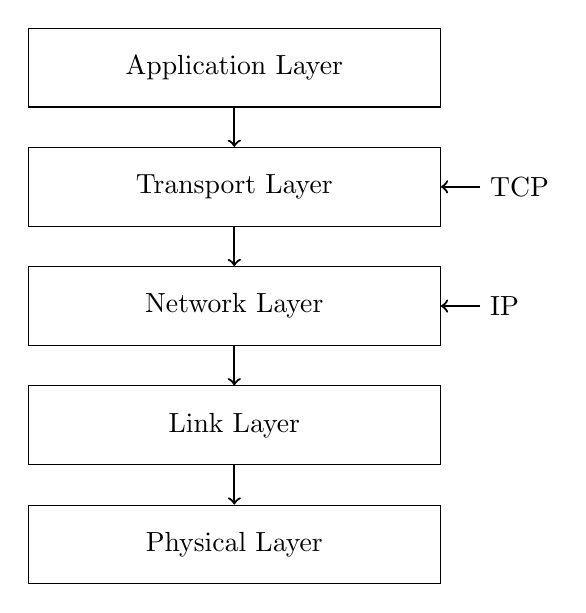
\begin{tikzpicture}[node distance=0.5cm]
        \tikzstyle{layer}=[rectangle, draw=black, fill=white, text width=5cm, text centered, minimum height=1cm]
        % Application Layer
        \node (app) [layer] {Application Layer};

        % Transport Layer
        \node (trans) [layer, below = of app] {Transport Layer};
        \node (tcp) [right = 0.5cm of trans] {TCP};

        % Network Layer
        \node (inet) [layer, below = of trans] {Network Layer};
        \node (ip) [right = 0.5cm of inet] {IP};

        % Link Layer
        \node (access) [layer, below = of inet] {Link Layer};
        % \node (eth) [below = 0.5cm of access] {Ethernet};
        % \node (wifi) [below = 0.5cm of eth] {Wi-Fi};

        % Physical Layer
        \node (phys) [layer, below = of access] {Physical Layer};

        % Arrows
        \draw[->,thick] (tcp) -- (trans);
        \draw[->,thick] (ip) -- (inet);
        \draw[->,thick] (app) -- (trans);
        \draw[->,thick] (trans) -- (inet);
        \draw[->,thick] (inet) -- (access);
        \draw[->,thick] (access) -- (phys);
    \end{tikzpicture}
    \caption{The TCP/IP Reference Model \cite{tcpip}}
    \label{fig:tcpip}
\end{figure}

When two computers want to send data to each other, they may use the \textbf{Internet Protocol} (IP) \cite{rfc791} directly. IP fragments data into blocks of data called \textit{packets} (also called datagrams) and transmits them from the source to the destination. The sources and destinations are computers identified by fixed length addresses. However, IP is a low-level protocol that does not interact directly with application data and may cause unreliable data transmission.

In the TCP/IP Reference Model \cite{tcpip}, the IP protocol works in the network layer, which is two layers below the application layer (see Figure \ref{fig:tcpip}). This layer provides an unreliable, connectionless delivery system (there is no direct connection between two hosts) which does not provide any functionality for error recovery for datagrams that are either duplicated, lost or arrive at the remote host in another order than they were sent. The transport layer, which is the layer above the network layer, is responsible for fixing the unreliable data transmission with transport protocols like \textbf{Transmission Control Protocol (TCP)} \cite{rfc793}. TCP is the most commonly used transport protocol on top of IP and includes strategies for packet ordering, retransmission, and maintaining data integrity.

TCP is a connection-oriented protocol, which means that before any data can be sent, a connection must be established between the two hosts. This connection is established by a three-way handshake between the two hosts. The first computer sends a packet with the SYN (a field in the TCP header) bit set to 1. The second computer responds with a packet with the SYN and ACK (another field in the TCP header) bits set to 1. The first computer then sends a packet with the ACK bit set to 1. Once the connection is established, the two hosts can start sending data to each other.

Now that we have established a connection between two hosts and have the ability to reliably send data across, we can further improve the transmission by using \textbf{Transport Layer Security (TLS)} \cite{rfc8446} (original \cite{rfc2246}). TLS protocol allows two hosts to communicate in a way that is designed to prevent eavesdropping, tampering, or message forgery. While TCP provides reliable data transmission, the data in the packets is unencrypted and can be read by anyone who has access to the network. This is acceptable when the data is not sensitive, but when the data is sensitive, TLS is used to \textit{encrypt} the data. TLS also provides \textit{authentication} of the remote host, which means that the remote host can be trusted to be the host it claims to be.

TLS is primarily used in a client/server setting where the client initiates the connection and the server responds. Setting up a TLS connection requires a handshake between the client and the server. At the end of the handshake, the client and the server have agreed upon a shared secret key which is used to encrypt the data, the encryption schemes and their parameters, and the client is also assured of the server's identity (not without issues \cite{rfc6962, tlsCertificateIssues}).

In this report, we discuss TLS 1.3 \cite{rfc8446}, which is the latest version of TLS in two sections. Section 1 covers the \textit{handshake protocol} in TLS 1.3. Section 2 discusses the \textit{record protocol} that uses the parameters established by the handshake protocol to protect traffic between the communicating hosts.



\section{Background}
\label{sec:background}
\subsection{Authenticated Encryption with Associated Data (AEAD)}
Cryptographic applications commonly require both confidentiality and message authentication. Confidentiality ensures that data is available only to those authorized to obtain it; usually it is realized through encryption.  Message authentication is the service that ensures that data has not been altered or forged by unauthorized entities; it can be achieved by using a Message Authentication Code (MAC). This service is also called data integrity. \textbf{Authenticated Encryption (AE)} \cite{ae} schemes ensure both data secrecy (confidentiality) and data integrity. These schemes can be constructed with either a \textbf{generic composition} that combines a CPA-secure cipher with a secure MAC, or to build them directly from a block cipher or a PRF without first constructing either a standalone cipher or MAC \cite{gradcourse}. The latter schemes are called \textbf{integrated schemes}. 

Let $(E, D)$ be a cipher and $(S, V)$ be a MAC. Let $k_{enc}$ be a cipher key and $k_{mac}$ be a MAC key. In a generic composition, these two primitives can be combined using two commonly used options: \textbf{Encrypt-then-MAC} and \textbf{MAC-then-Encrypt}. In the first option, the plaintext is encrypted using the cipher and the resulting ciphertext is authenticated using the MAC. In the second option, the plaintext is authenticated using the MAC and the resulting MAC tag is encrypted using the cipher (see Figure \ref{fig:encrypt-then-mac} and Figure \ref{fig:mac-then-encrypt}). Only the first method is secure for every combination of CPA-secure cipher and secure MAC. The intuition is that the MAC on the ciphertext prevents any tampering with the ciphertext. The second method is known to have attacks in some cases \cite{gradcourse}. 

TLS uses a nonce-based \textbf{Authenticated Encryption with Associated Data (AEAD)} \cite{aead} cipher to encrypt and authenticate packets. AEAD schemes are an extension of AE schemes (discussed above) that allow the sender to send additional data along with the message. This additional data is called the \textbf{associated data} (AD) and its integrity is protected by the ciphertext, but its secrecy is not. The associated data is required to set context; for example in a networking protocol, authenticated encryption protects the packet body, but the header must be transmitted in the clear so that the network can route the packet to its intended destination \cite{gradcourse}. Nonetheless, we want to ensure header integrity so that a malicious adversary can't get away with tampering the header. This header is provided as the associated data input to the AEAD encryption scheme. Secondly, the encryption scheme takes an additional input nonce $\mathcal{N}$, which is a random value that is used only once. This nonce ensures that the same plaintext is never encrypted to the same ciphertext. 
% \newpage
\begin{figure}[t]
  \centering
  \begin{subfigure}[b]{0.4\textwidth}
    \centering
    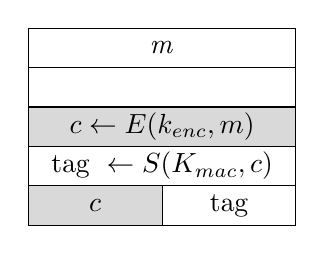
\begin{tikzpicture}[node distance=0 cm,outer sep = 0pt,inner sep = 2pt]
      \tikzset{field/.style={align=center,shape=rectangle,minimum height=0.5cm,minimum width=17mm,draw}}
      \tikzset{largefield/.style={align=center,shape=rectangle,minimum height=0.5cm,minimum width=34mm,draw}}
    
        \node [largefield] (message) {\textit{m}};
        \node [largefield, below=of message] (empty) { };
        \node [largefield,below=of empty,fill=gray!30] (enc) {$c \leftarrow E(k_{enc}, m)$};
        \node [largefield,below=of enc] (mac) {$\text{tag } \leftarrow S(K_{mac}, c)$};
        \node [field,below=of mac, xshift=-8.5mm, fill=gray!30] (cipher) {$c$};
        \node [field,below=of mac, xshift=8.5mm] (tag) {tag};
    \end{tikzpicture}
    \caption{Encrypt-then-MAC}
    \label{fig:encrypt-then-mac}
  \end{subfigure}
  \begin{subfigure}[b]{0.4\textwidth}
    \centering
    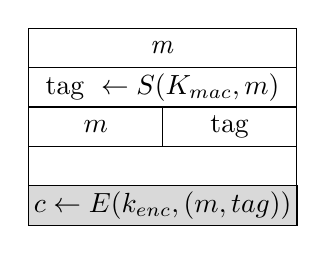
\begin{tikzpicture}[node distance=0 cm,outer sep = 0pt,inner sep = 2pt]
        \tikzset{field/.style={align=center,shape=rectangle,minimum height=0.5cm,minimum width=17mm,draw}}
        \tikzset{largefield/.style={align=center,shape=rectangle,minimum height=0.5cm,minimum width=34mm,draw}}
    
        \node [largefield] (message) {\textit{m}};
        \node [largefield,below=of message] (mac) {$\text{tag } \leftarrow S(K_{mac}, m)$};
        \node [field,below=of mac, xshift=-8.5mm] (pkt-m) {$m$};
        \node [field,below=of mac, xshift=8.5mm] (tag) {tag};
        \node [largefield, below=of pkt-m, xshift=8.5mm] (empty) { };
        \node [largefield,below=of empty,fill=gray!30] (enc) {$c \leftarrow E(k_{enc}, (m, tag))$};
  
    \end{tikzpicture}
    \caption{MAC-then-Encrypt}
    \label{fig:mac-then-encrypt}
  \end{subfigure}
  \label{fig:encrypt-then-mac-mac-then-encrypt}
  \caption{Two different ways to combine a cipher and a MAC.}
  \hrulefill
\end{figure}

\section{TLS Handshake Protocol}
\label{sec:handshake}
For consistency with the notation, we let P play the role of the client and Q play the role of the server. P and Q wish to setup a secure session. 

\textbf{TLS 1.3} supports both one-sided and mutual authentication. In most cases, authentication for the client is optional. In the notation, $(E_s , D_s)$ is a symmetric encryption scheme that provides authenticated encryption, such as AES-128 in GCM mode.  Algorithm $S$ refers to a MAC signing algorithm, such as HMAC-SHA256. Algorithms $Sig_P(\cdot )$ and $Sig_Q(\cdot )$ sign the provided data using P's or Q's signing keys. Finally, the hash functions $H_1, H_2$ are used to derive symmetric keys. They are built from HKDF (Apppendix I) with hash functions such as SHA-256. The notations are taken from \cite{gradcourse}.

The cipher-suites which determine the symmetric encryption scheme, the hash function in the MAC signing algorithm and HKDF are negotiated during the handshake. The cipher-suites are defined in \cite{rfc8446}. They are specified in Table \ref{tab:ciphersuites}. 

% TLS uses \textbf{Authenticated encryption} \cite{ae} that is a form of encryption that, in addition to providing confidentiality for the plaintext that is encrypted, provides a way to check its integrity and authenticity. \textbf{Authenticated Encryption with Associated Data (AEAD)} \cite{aead}, adds the ability to check the integrity and authenticity of some Associated Data (AD), also called "additional authenticated data", that is not encrypted.

% Many applications use an encryption method and a MAC together to provide both of those security services, with each algorithm using an independent key. More recently, the idea of providing both security services using a single cryptoalgorithm has become accepted \cite{rfc5116}. In this concept, the cipher and MAC are replaced by an Authenticated Encryption with Associated Data (AEAD) algorithm \cite{aead}.




\begin{table}[ht]
  \centering
  \begin{tabular}{|l|l|}
    \hline Description & Value \\
    \hline 
    TLS\_AES\_128\_GCM\_SHA256 & $\{0\times13,0\times01\}$ \\
    \hline TLS\_AES\_256\_GCM\_SHA384 & $\{0\times13,0\times02\}$ \\
    \hline TLS\_CHACHA20\_POLY1305\_SHA256 & $\{0\times13,0\times03\}$ \\
    \hline TLS\_AES\_128\_CCM\_SHA256 & $\{0\times13,0\times04\}$ \\
    \hline TLS\_AES\_128\_CCM\_8\_SHA256 & $\{0\times13,0\times05\}$ \\
    \hline
  \end{tabular}
  \caption{Cipher-Suites \cite{rfc8446}. Cipher suite names follow the naming convention: CipherSuite TLS\_AEAD\_HASH = VALUE;}
  \label{tab:ciphersuites}
\end{table}



\textbf{The protocol.} The handshake protocol 
% \begin{align*}
%     & \textbf { ClientHello } \\
%     & u:=g^\alpha, \mathcal{N}_{\mathrm{c}}, offer \\
%     & \textbf { ServerHello } \\
%     & v:=g^\beta, \mathcal{N}_{\mathrm{s}}, \text { mode } \\ 
%     & c_1:=E_{\mathrm{s}}\left(k_{\mathrm{sh}}, \text { CertReqest }\right) \\ 
%     & c_2:=E_{\mathrm{s}}\left(k_{\mathrm{sh}}, \operatorname{Cert}_Q\right) \\ 
%     & c_3:=E_{\mathrm{s}}\left(k_{\mathrm{sh}}, \text { Sig }\right. \\ 
%     & \left.c_4\left(u, \mathcal{N}_{\mathrm{c}}, \text { offer }, v, \mathfrak{N}_{\mathrm{s}}, \text { mode }, c_1, c_2\right)\right) \\ 
%     & c_4=E_{\mathrm{s}}\left(k_{\mathrm{sh}}, S\left(k_{\mathrm{sm}},\left(u, \mathfrak{N}_{\mathrm{c}}, \text { offer }, v, \mathfrak{N}_{\mathrm{s}}, \text { mode }, c_1, c_2, c_3\right)\right)\right) \\
%     & \left(k_{\mathrm{sh}}, k_{\mathrm{sm}}, k_{\mathrm{ch}}, k_{\mathrm{cm}}\right):=H_1\left(g^{\alpha \beta}, u, \mathcal{N}_{\mathrm{c}}, \text { offer }, v, \mathcal{N}_{\mathrm{s}}, \text { mode }\right) \\
%     & \left(k_{\mathrm{c} \rightarrow \mathrm{s}}, k_{\mathrm{s} \rightarrow \mathrm{c}}\right):=H_2\left(g^{\alpha \beta}, u, \mathcal{N}_{\mathrm{c}}, \text { offer, } v, \mathfrak{N}_{\mathrm{s}}, \text { mode }, c_1, \ldots, c_4\right) \\
%     & \text { ClientKeyExchange } \\
% \end{align*}

% \begin{figure}[ht]
%     \centering
%     \begin{tikzpicture}[block/.style={draw,minimum width=2cm,minimum height=1cm}, font=\sffamily] 
%     \node[block](C) {Client}; 
%     \node[block,right=9cm of C](S) {Server}; 
%     \draw[-latex] (C.15) -- (S.165)
%     node[midway,above]{Request(GET,POST,PUT,DELETE,HEAD,OPTION)}; 
%     \draw[-latex] (S.195) -- (C.-15) node[midway,above]{
%       $\begin{aligned}
%         & \textbf { ServerHello } \\
%         & v:=g^\beta, \mathcal{N}_{\mathrm{s}}, \text { mode } \\ 
%         & c_1:=E_{\mathrm{s}}\left(k_{\mathrm{sh}}, \text { CertReqest }\right) \\ 
%         & c_2:=E_{\mathrm{s}}\left(k_{\mathrm{sh}}, \operatorname{Cert}_Q\right) \\ 
%         & c_3:=E_{\mathrm{s}}\left(k_{\mathrm{sh}}, \text { Sig }\right. \\ 
%         & \left.c_4\left(u, \mathcal{N}_{\mathrm{c}}, \text { offer }, v, \mathfrak{N}_{\mathrm{s}}, \text { mode }, c_1, c_2\right)\right) \\ 
%         & c_4=E_{\mathrm{s}}\left(k_{\mathrm{sh}}, S\left(k_{\mathrm{sm}},\left(u, \mathfrak{N}_{\mathrm{c}}, \text { offer }, v, \mathfrak{N}_{\mathrm{s}}, \text { mode }, c_1, c_2, c_3\right)\right)\right) \\
%         & \left(k_{\mathrm{sh}}, k_{\mathrm{sm}}, k_{\mathrm{ch}}, k_{\mathrm{cm}}\right):=H_1\left(g^{\alpha \beta}, u, \mathcal{N}_{\mathrm{c}}, \text { offer }, v, \mathcal{N}_{\mathrm{s}}, \text { mode }\right) \\
%         & \left(k_{\mathrm{c} \rightarrow \mathrm{s}}, k_{\mathrm{s} \rightarrow \mathrm{c}}\right):=H_2\left(g^{\alpha \beta}, u, \mathcal{N}_{\mathrm{c}}, \text { offer, } v, \mathfrak{N}_{\mathrm{s}}, \text { mode }, c_1, \ldots, c_4\right) \\
%       \end{aligned}$
%     }; 
%     \end{tikzpicture}
%     \caption{TLS Handshake Sequence}
%     \label{fig:handshake}
%   \end{figure}

\section{TLS Record Protocol}
\label{sec:record}
The TLS record protocol \cite{rfc8446} uses the parameters established by the handshake protocol to protect traffic between the communicating peers. The record protocol divides traffic up into a series of records, each of which is independently protected
using the traffic keys.
\section{Packet Capture}
We captured a TLS packet sent Facebook. This packet contains to ClientHello message described in Handshake Protocol section. The yellow highlight marks the beginning of the TLS packet with 16 marking the record layer content type as Handshake. The cyan highlighted portion is the random nonce sent by the client to the server. The blue highlights the ciphersuites the client can use to for symmetric encryption.
\begin{figure}[h!]
    \includegraphics*[width=\textwidth]{images/clientHello.png}
\end{figure}
% \section{Applications}
% \input{sections/04_applications.tex}

\newpage
\bibliographystyle{IEEEtran}
\bibliography{bibliography.bib}

\end{document}